
%Este arquivo deve ser alterado pelos integrantes da respectiva equipe com o conteudo indicado abaixo.
\subsection{Limitação do tamanho da janela do destinatário}
%Equipe: Sergio Vieira, Wilson

% Livro: Seção 5.3.1, p.136

%Inserir no arquivo \textbf{janela\_destino.tex} a descrição da influência do tamanho da janela 
%do detinatário no modelo TCP.

A modificação final do modelo é incluir uma situação na qual o destinatário pode limitar o tamanho da janela do remetente. Isto ocorre quando o destinatário pode processar pacotes até uma taxa de recepção máxima, neste caso, o remetente não deve transmitir uma rajada de pacotes a uma taxa que prejudique a recepção do destinatário. Em consequência disto, durante o período sem indicação de perda, o tamanho da janela pode crescer até um tamanho máximo (Figura \ref{fig:max}). 

\begin{figure}[ht]
  \centering
  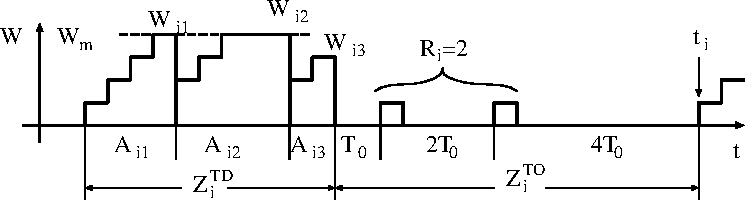
\includegraphics[scale=0.8]{figs/windowmax.pdf}
  \caption{Evolução do tamanho da janela limitada por um valor m
áximo}
  \label{fig:max}
\end{figure}

Denota-se $W_m$ como o limite imposto pelo destinatário para o tamanho máximo da janela e $W_u$ como o tamanho da janela sem restrições. Se $E[W_u]$ é menor que o limite da janela do destinatário, isto é, se $E[W_u]<W_m$, então a limitação da janela de recepção tem um efeito insignificante a longo prazo na vazão média do TCP, assim, como demonstrado anteriormente, $E[W_u]$
 é dado pela equação \ref{eq:wmax}. 

\begin{equation} \label{eq:wmax}
E[W_u]= 1 + \sqrt{\frac{8}{3p} - \frac{5}{3}}
\end{equation}

Se, entretanto, $W_m \leq E[W_u]$, a janela é considerada como sendo $E[W] \approx E[W_m]$. Desta maneira, como pode ser observado na Figura \ref{fig:limit}, em um período $Z_i^{TD}$ e em cada $TDP_i$, o tamanho da janela cresce linearmente até atingir um valor máximo $W_m$ em $U_i$ rodadas e permanece constante durante $V_i$ rodadas.

\begin{figure}[ht]
  \centering
  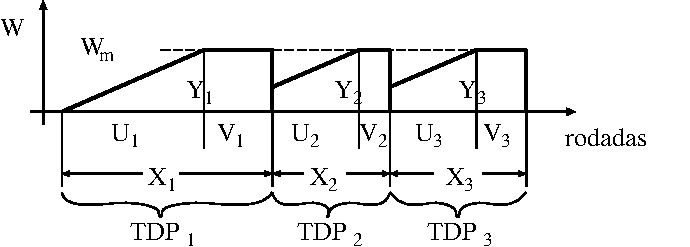
\includegraphics[scale=0.8]{figs/limit.pdf}
  \caption{Retransmissão rápida com limitação da janela}
  \label{fig:limit}
\end{figure}

Para determinar a quantidade de pacotes enviados no período $X_i$ basta calcular a área da figura formada durante $U_i$ rodadas (trapézio) mais a área da figura durante $V_i$ rodadas (retângulo). Assim a quantidade de pacotes $Y_i$ é dada por \ref{eq:pkts}.

\begin{equation} \label{eq:pkts}
Y_i=\frac{U_i(W_m + \frac{W_m}{2})}{2} + V_i \cdot W_m
\end{equation}

Desenvolvendo, tem-se:

\begin{align} \label{eq:EY1}
  \nonumber E[Y] &= \frac{W_mE[U]+\frac{W_mE[U]}{2}}{2} + W_mE[V]\\
  \nonumber     &= \frac{\frac{2W_mE[U]+W_mE[U]}{2}}{2} + W_mE[V]\\
       &= \frac{3W_mE[U]}{4} + W_mE[V]
\end{align}

Quando ocorre uma triplo ACK, a janela $W_m$ é dividida pela metade, assim, para que seu valor novamente atinja $W_m$ ela deve ser incrementada em $\frac{W_m}{2}$. No entanto, este acréscimo deve ocorrer dentro da rodada $U_i$, assim $W_m = \frac{W_m}{2} + U_i$, $\forall i \geq 2$ , desenvolvendo tem-se:

\begin{align} \label{eq:EY2}
  \nonumber W_m &= \frac{W_m}{2} + E[U]\\
  \nonumber     &= \frac{W_m+2E[U]}{2}\\
  \nonumber	2W_m - W_m &= 2E[U]\\
      E[U] &= \frac{W_m}{2}
\end{align} 

Substituindo $E[U]$ em \ref{eq:EY1}, tem-se:

\begin{align} \label{eq:EY3}
  \nonumber E[Y] &= \frac{3W_mE[U]}{4} + W_mE[V]\\
  \nonumber     &= \frac{3W_m\cdot \frac{W_m}{2}}{4} + W_mE[V]\\
      &= \frac{3W_m^2}{8} + W_mE[V]
\end{align}

Como o número de pacotes enviados em cada $TDP_i$ não se altera mesmo como um tamanho de janela limitado, o valor esperado de pacotes enviados é dado por $E[Y]=\frac{1-p}{p} + W_m$. Substituindo $E[Y]$ em \ref{eq:EY3} tem-se:

\begin{align} \label{eq:EY4}
  \nonumber \frac{1-p}{p} + W_m &= \frac{3}{8}W_m^2+W_mE[V]\\
  \nonumber \frac{ \frac{1-p}{p} + W_m }{W_m} &= \frac{ \frac{3}{8}W_m^2+W_mE[V] }{W_m}\\
  \nonumber \frac{1-p}{pW_m} + 1 &= \frac{3}{8}W_m+E[V]\\
  E[V] &= \frac{1-p}{pW_m} + 1 - \frac{3}{8}W_m
\end{align}

Finalmente, uma vez que $X_i=U_i+V_i$, temos:

\begin{align} \label{eq:EX}
  \nonumber E[X] &= E[U] + E[V]\\
  \nonumber &= \frac{W_m}{2} + \frac{1-p}{pW_m} + 1 - \frac{3}{8}W_m\\
  \nonumber &= \frac{W_m}{2} - \frac{3}{8}W_m + \frac{1-p}{pW_m} + 1\\
  \nonumber &= W_m(\frac{1}{2} - \frac{3}{8}) + \frac{1-p}{pW_m} + 1\\
  \nonumber &= \frac{1}{8}W_m + \frac{1-p}{pW_m} + 1\\
\end{align}

Para determinar a vazão do TCP levando-se em conta o tamanho máximo da janela substitui-se os valores de $E[X]$ na equação abaixo:

\begin{align} \label{eq:EX2}
  \nonumber  \overline{X}(p) &= \frac{\frac{1-p}{p}+E[W]+Q(E[W])\frac{1}{1-p}}{RTT(E[X]+1)+Q(E[W])T_0\frac{f(p)}{1-p}}\\
  \nonumber  \overline{X}(p) &= \frac{\frac{1-p}{p}+W_m+Q(W_m)\frac{1}{1-p}}{RTT(\frac{W_m}{8}+\frac{1-p}{pW_m}+1)+Q(E[W])T_0\frac{f(p)}{1-p}}
\end{align}

Portanto, o modelo completo da vazão do TCP é caracterizado por:

\begin{equation*}
\overline{X}(p)= 
\begin{cases} \dfrac{\frac{1-p}{p}+E[W]+Q(E[W])\frac{1}{1-p}}{RTT(\frac{E[W]}{2}+1)+Q(E[W])T_0\frac{f(p)}{1-p}}, & E[W_u]<W_m \\
\dfrac{\frac{1-p}{p}+W_m+Q(E[W_m])\frac{1}{1-p}}{RTT(\frac{W_m}{8}+\frac{1-p}{pW_m}+1)+Q(E[W_m])T_0\frac{f(p)}{1-p}}, & E[W_u]\approx W_m
\end{cases}
\label{eq:03}
\end{equation*}
